\subsection{Peak performance}
\label{subsec:peak_fp}
Rosa's nodes are equipped with dual-socket Intel Xeon E5-2650 v3 processors, 10 cores and AVX2 units that operates with 256-bit vectors\cite{intel-e5-2650v3,usi-rosa-hardware}. Haswell micro-architecture have two 256-bit FMA instructions per cycle meaning that each core performs four double-precision at 2.30~GHz \cite{intel-optimization-manual}.

The Rosa documentation (and also the output from command \texttt{sinfo} \ref{lst:sinfo}) shows 42 compute nodes (icsnode01--icsnode42).\cite{usi-rosa-hardware} \\ 
The calculations for the aggregate peak throughput for the partition is written in the provided file \href{run:../src/2-Performance-characteristics/01/INTEL_XEON_E5-2650.txt}{[INTEL\_XEON\_E5-2650.txt]} in the \href{run:../src/2-Performance-characteristics/02/}{02} folder and reported here below:

\lstinputlisting[
    caption={Peak throughput breakdown for Intel Xeon E5-2650 v3},
    captionpos=b,
    label={lst:e5-2650-peak},
]{../src/2-Performance-characteristics/01/INTEL_XEON_E5-2650.txt}


\subsection{Memory Hierarchies}
\label{subsec:memory_hierarchy}

In order to study the memory hierarchy of Rosa compute nodes, I used the commands: \texttt{lscpu}, \texttt{cat /proc/meminfo}, and \texttt{hwloc-ls}. The complete output files are available in the submission in the folder \href{run:../src/2-Performance-characteristics/02/}{02}.

The results are summarized in Table~\ref{tab:memory_hierarchy}.

\begin{table}[h]
    \centering
    \begin{tabular}{|l|r|}
    \hline
    \textbf{Component} & \textbf{Size} \\
    \hline
    Main memory (total) & 62 GB \\
    Main memory (per NUMA node) & 31 GB \\
    L3 cache (shared per socket) & 25 MB \\
    L2 cache (per core) & 256 KB \\
    L1d cache (per core) & 32 KB \\
    L1i cache (per core) & 32 KB \\
    \hline
    \end{tabular}
    \caption{Memory hierarchy of Rosa compute node}
    \label{tab:memory_hierarchy}
\end{table}

The graphical representation of the memory hierarchy is shown in Figure~\ref{fig:memory_topology}.

\begin{figure}[h]
\centering
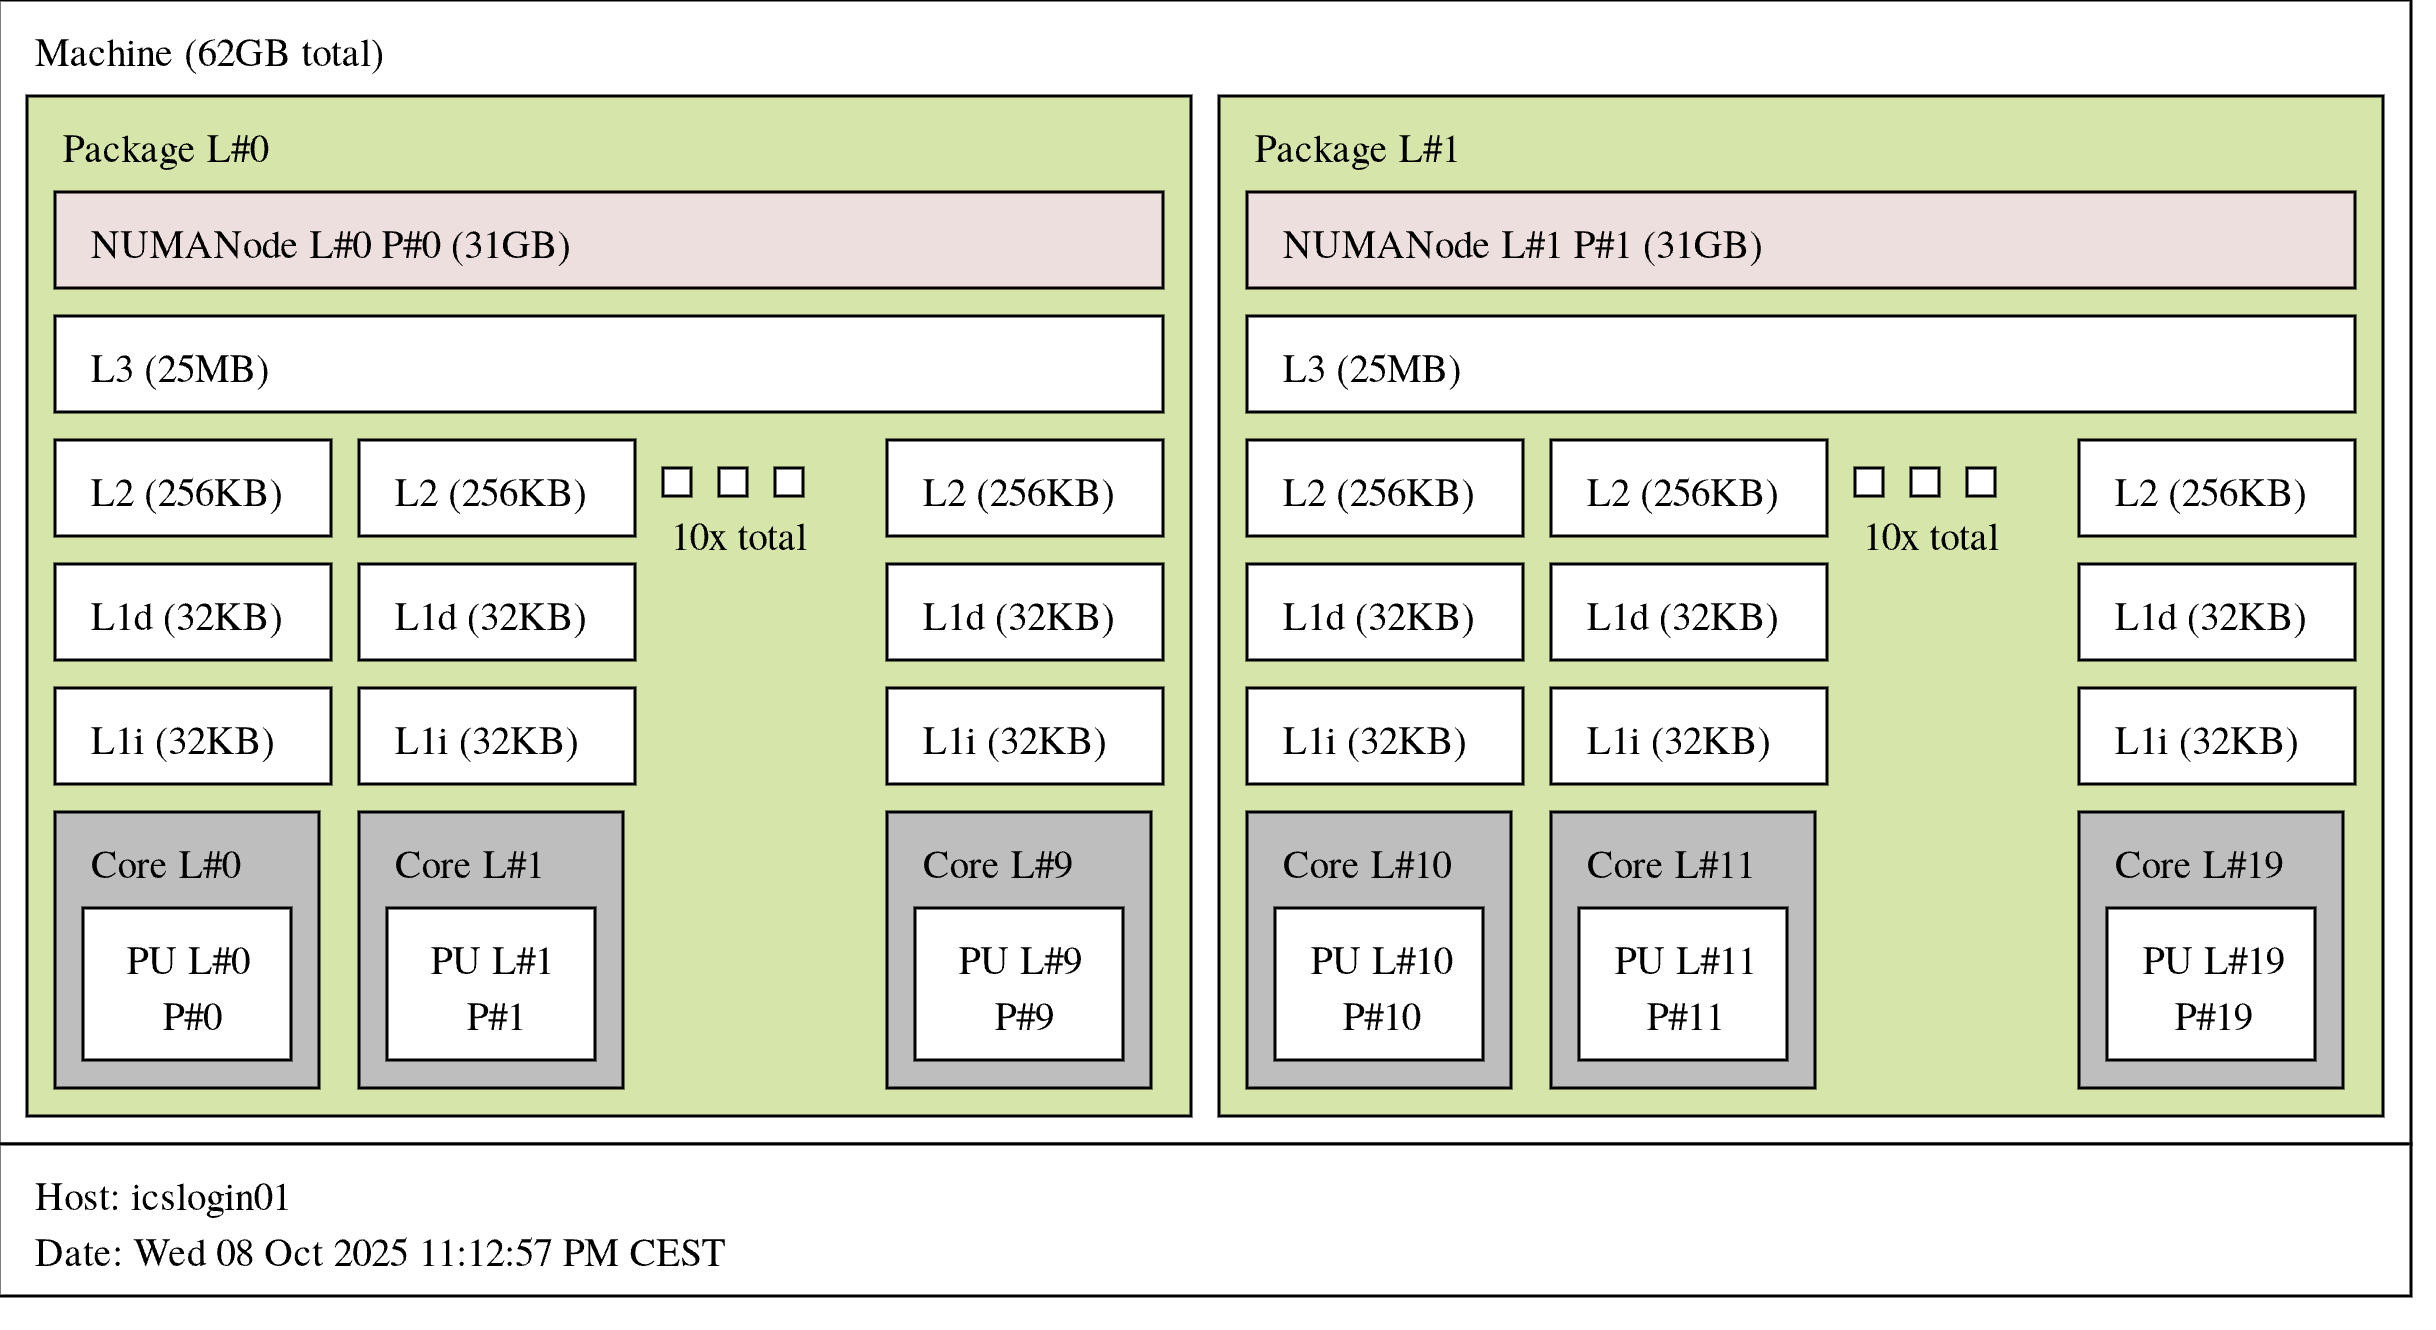
\includegraphics[width=0.9\textwidth]{../src/2-Performance-characteristics/02/XEON_E5-2650.png}
\caption{Graphical representation of Rosa node topology generated by command \texttt{hwloc-ls}.}
\label{fig:memory_topology}
\end{figure}


\subsection{Bandwidth: STREAM benchmark}
\label{subsec:stream}

The STREAM benchmark was executed on a single core of a Rosa consisting of four simple vector operations: Copy, Scale, Add, and Triad.

As required I runned the command:
\begin{verbatim}
    gcc -O3 -march=native -DSTREAM_TYPE=double -DSTREAM_ARRAY_SIZE=128000000 
        -DNTIMES=20 stream.c -o stream_c.exe
\end{verbatim}

So the array size is configured to 128,000,000 elements (~3GB) which significantly exceeds the L3 cache size (25MB), ensuring that the operations always "fall" out of the cache and therefore forcing the use main memory. This is done to \textbf{measure the bandwidth of main memory rather than cache performance.} Each kernel has been executed 20 times, and the best time (excluding the first iteration) I used to compute the reported bandwidth.

The complete output is available in the submission folder. The key results are shown below:

\lstinputlisting[
    caption={STREAM benchmark output on Rosa compute node (single-core)},
    captionpos=b,
    label={lst:stream-output},
]{../src/2-Performance-characteristics/03/slurm-52026.out}

The Copy operation shows substantially higher bandwidth (approximately 19GB/s) compared to the others.

The \textbf{Triad kernel bandwidth} of approximately 12.3 GB/s will be the average representative as memory bandwidth for a single core on Rosa compute nodes.

\subsection{Performance model: A simple roofline model}
\label{subsec:roofline}

Using the values obtained from the previous sections:
\begin{itemize}
    \item Peak performance per core: $P_{max} = 36.8$ GFlops/s (Section~\ref{subsec:peak_fp})
    \item Memory bandwidth per core: $b_{max} = 12.3$ GB/s (Section~\ref{subsec:stream})
\end{itemize}

The ridge point (performance transitions from memory-bound to compute-bound) occurs at:
\[
I_{ridge} = \frac{P_{max}}{b_{max}} = \frac{36.8}{12.3} \approx 2.99~\mathrm{Flops/Byte}
\]

\begin{figure}[h]
    \centering
    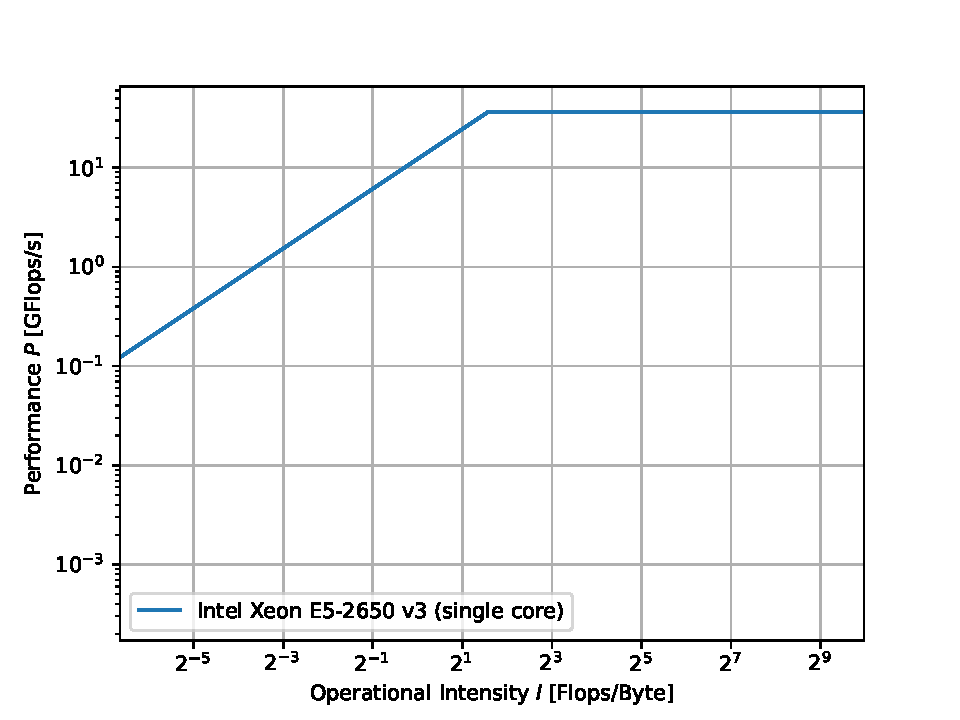
\includegraphics[width=0.9\textwidth]{../src/2-Performance-characteristics/04/roofline.pdf}
    \caption{Roofline model for Intel Xeon E5-2650 v3 (single core) on Rosa compute node.}
    \label{fig:roofline}
\end{figure}
